\subsection{Premi::Front-End}
	\subsubsection*{Informazioni sul package}
		\begin{figure}[h]
			\centering
			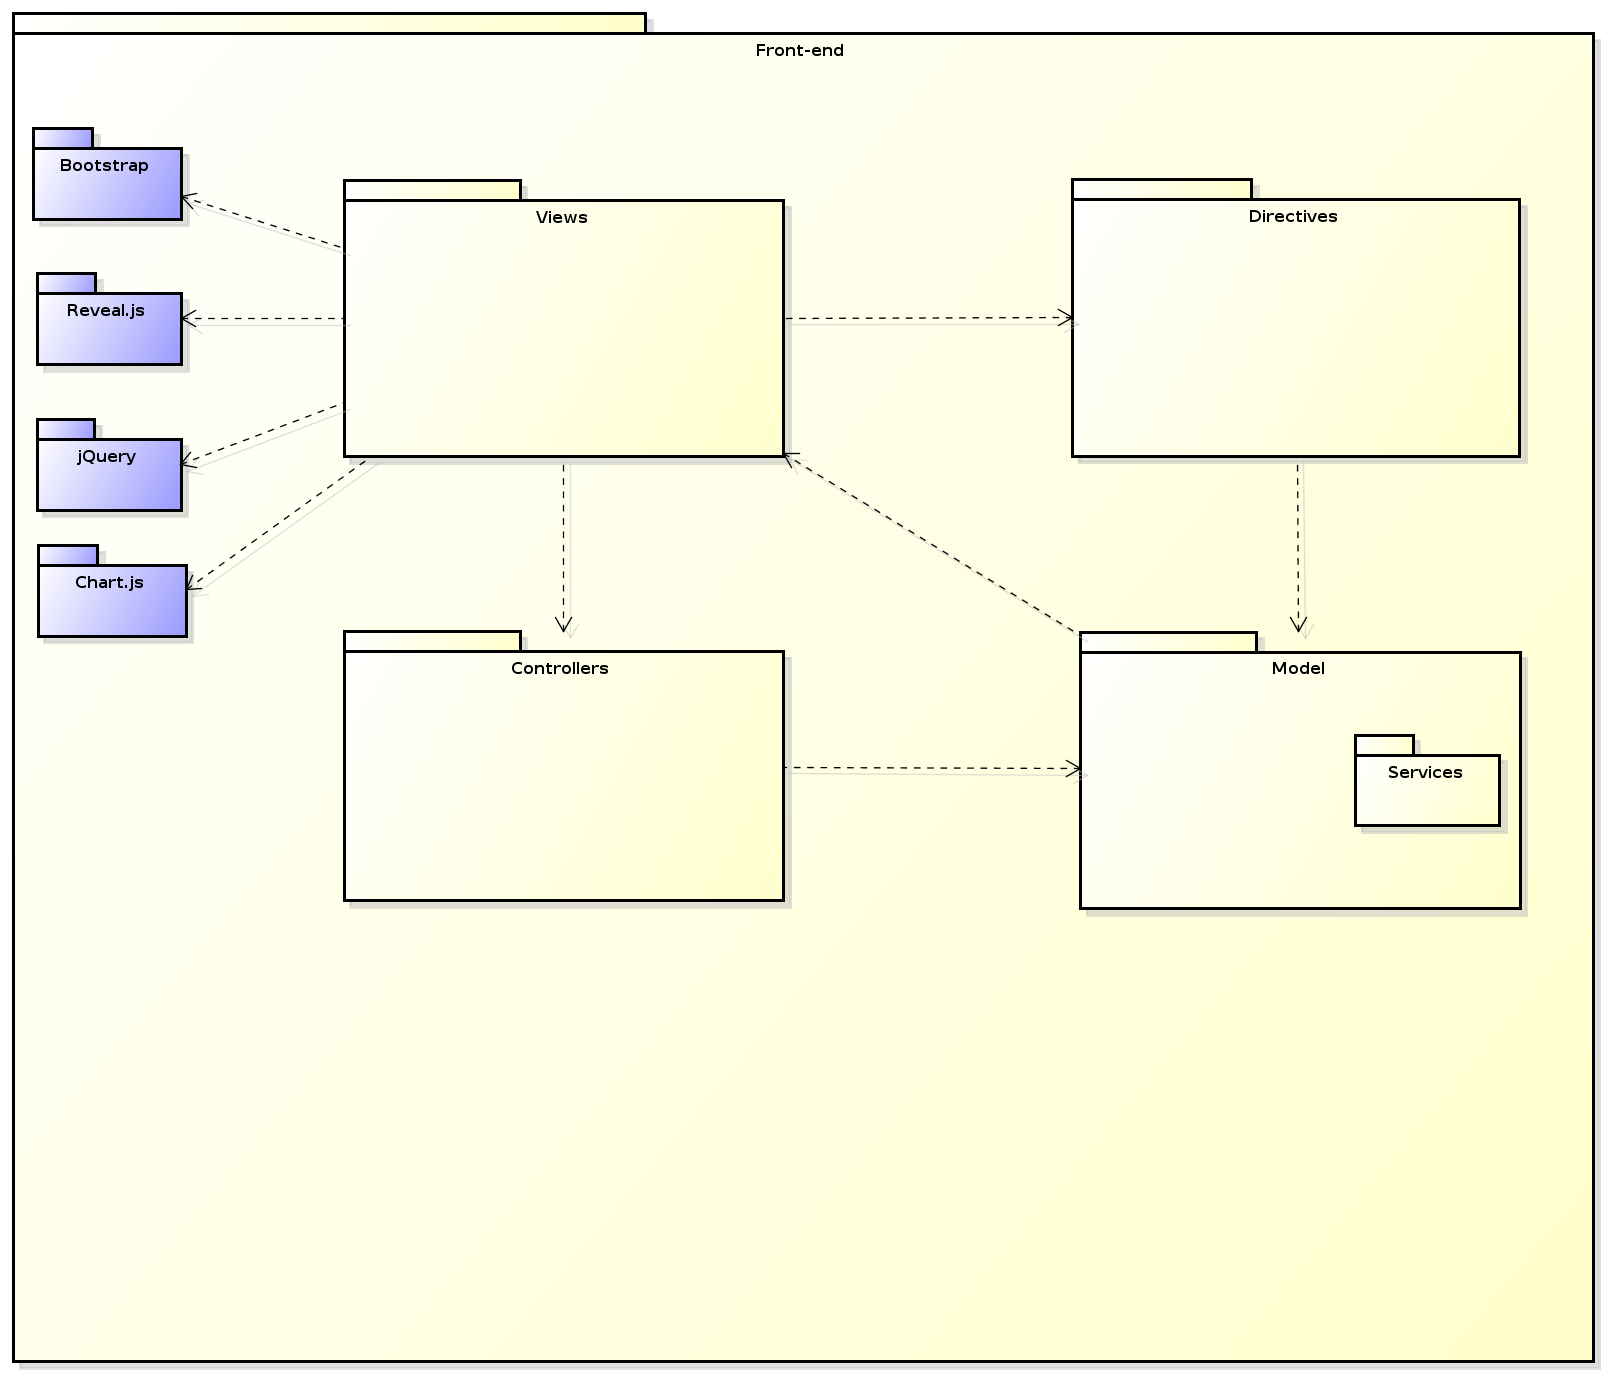
\includegraphics[width=\linewidth]{img/front-end-package}
			\caption[Premi::Front-End]{Premi::Front-End}
		\end{figure}
		Il package contiene le varie componenti della parte di front-end dell'applicazione.

		\subsubsection*{Package contenuti:}
			\begin{itemize}
				\item \textbf{View:} Package contenente le views della componente front-end dell'applicazione;
				\item \textbf{Directives:} Package contenente le directives che compongono la view;
				\item \textbf{Model:} Package che definiscono la business logic dell'applicazione;
				\item \textbf{Controller:} Package contenente i controller della parte front-end dell'applicazione.
			\end{itemize}

		\subsection{Premi::Front-End::Model}
				\subsubsection*{Informazioni sul package}
		\begin{figure}[h]
			\centering
			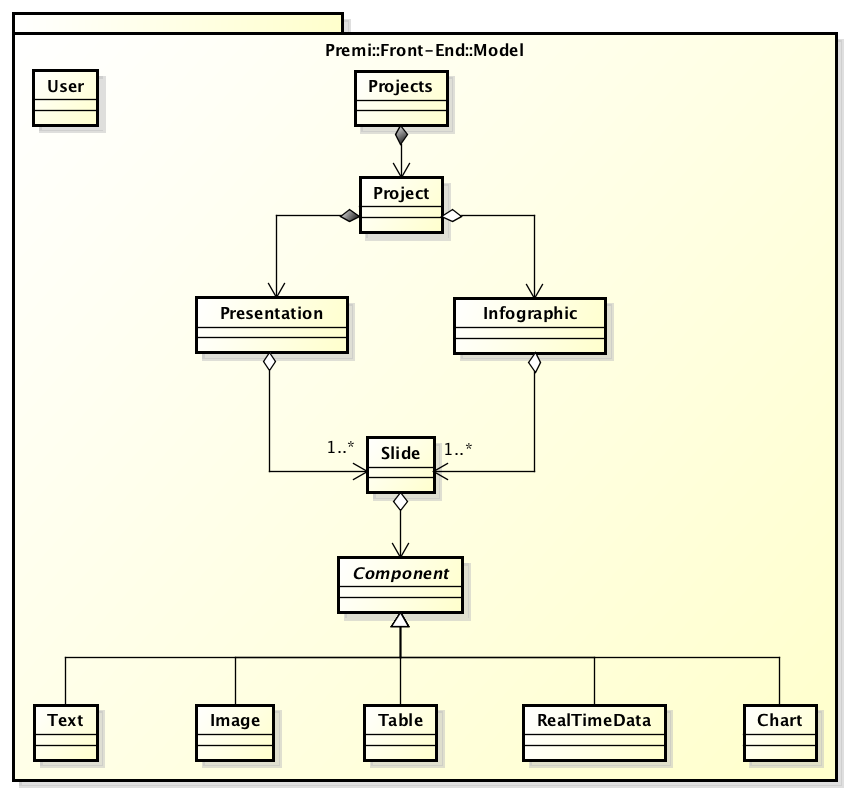
\includegraphics[width=0.9\linewidth]{img/front-end_model}
			\caption[Premi::Front-End::Model]{Premi::Front-End::Model}
		\end{figure}
		Il package serve per mantenere i dati relativi al \textit{\gls{front-end}} e tutta la loro logica di \gls{business}.

	\subsubsection*{Classi contenute}
		\begin{itemize}
		 \item Premi::Front-End::Model::Projects:
			\begin{itemize}
				\item \textbf{Descrizione}:classe per la gestione di una collezione di progetti.Un progetto racchiude una presentazione e zero o più infografiche.
				\item \textbf{Relazioni con altre classi}:
				\begin{itemize}
					\item Premi::Front-End::Model::Project.
				\end{itemize}
			\end{itemize}
		\item  Premi::Front-End::Model::Project: 
			 \begin{itemize}
				\item \textbf{Descrizione}: classe per la gestione di un progetto.
				\item \textbf{Relazioni con altre classi}:
				\begin{itemize}
					\item Premi::Front-End::Model::Presentation.
					\item Premi::Front-End::Model::Infographic.
				\end{itemize}
			\end{itemize}
		 \item  Premi::Front-End::Model::Infographic:
			\begin{itemize}
				\item \textbf{Descrizione}: classe per la gestione di una \gls{infografica}. Un'\gls{infografica} ha il compito di raggruppare piu \gls{slide} in un \gls{template} grafico scelto dall'utente in un ordine impostabile di volta in volta.
				\item \textbf{Relazioni con altre classi}:
				\begin{itemize}
					\item Premi::Front-End::Model::\gls{Slide}.
				\end{itemize}
			\end{itemize}
		 \item   Premi::Front-End::Model::Presentation:
			\begin{itemize}
				\item \textbf{Descrizione}: classe per la gestione di una presentazione. Una presentazione raggruppa più \gls{slide}. Per la visualizzazione delle presentazioni è stato scelto di utilizzare il \gls{framework} \gls{Reveal.js} che permette di avere una visualizzazione a griglia, di conseguenza una presentazione deve memorizzare anche le coordinate delle sue \gls{slide}.
				\item \textbf{Relazioni con altre classi}:
				\begin{itemize}
					\item Premi::Front-End::Model::\gls{Slide}.
				\end{itemize}
			\end{itemize}
		 \item Premi::Front-End::Model::\gls{Slide}: Classe per la gestione di una \gls{slide}.
			\begin{itemize}
				\item \textbf{Descrizione}: classe per la gestione di una \gls{slide}.
				\item \textbf{Relazioni con altre classi}:
				\begin{itemize}
					\item Premi::Front-End::Model::Component.
				\end{itemize}
			\end{itemize}
		 \item  Premi::Front-End::Model::Component: 
			\begin{itemize}
				\item \textbf{Descrizione}: Classe astratta concretizzata ed estesa dalle varie componenti implementando il pattern \textit{composite} per fare si che elementi foglia e collezione vengano trattati allo stesso modo. Nello specifico, una tabella rappresenta un aggregato di altre componenti.
			\end{itemize}
		 \item  Premi::Front-End::Model::Text:
			\begin{itemize}
				\item \textbf{Descrizione}: classe per la gestione di un elemento testuale e delle sue proprietà di formattazione. Concretizza ed estende Premi::Front-End::Model::Component.
				\item \textbf{Relazioni con altre classi}:
				\begin{itemize}
					\item Premi::Front-End::Model::Component.
				\end{itemize}
			\end{itemize}
		 \item  Premi::Front-End::Model::Image:
			\begin{itemize}
				\item \textbf{Descrizione}: lasse per la gestione di un elemento di tipo immagine.
				\item \textbf{Relazioni con altre classi}:
				\begin{itemize}
					\item Premi::Front-End::Model::Component.
				\end{itemize}
			 \end{itemize}
		 \item  Premi::Front-End::Model::Table:
			\begin{itemize}
				\item \textbf{Descrizione}: classe per la gestione di una tabella. Una tabella può contenere altre componenti che concretizzano la classe Premi::Front-End::Model::Component.
				\item \textbf{Relazioni con altre classi}:
				\begin{itemize}
					\item Premi::Front-End::Model::Component.
				\end{itemize}
			 \end{itemize}
		 \item  Premi::Front-End::Model::RealTimeData:
			\begin{itemize}
				\item \textbf{Descrizione}: classe per la gestione di componenti che si aggiornano in tempo reale con cadenza personalizzabile.
				\item \textbf{Relazioni con altre classi}:
				\begin{itemize}
					\item Premi::Front-End::Model::Component.
				\end{itemize}
			 \end{itemize}
		 \item  Premi::Front-End::Model::Chart: 
			\begin{itemize}
				\item \textbf{Descrizione}: classe per la gestione dei dati necessari per disegnare un grafico.
				\item \textbf{Relazioni con altre classi}:
				\begin{itemize}
					\item Premi::Front-End::Model::Component.
				\end{itemize}
			 \end{itemize}
		 \item  Premi::Front-End::Model::User:
			\begin{itemize}
				\item \textbf{Descrizione}: classe per la gestione degli utenti.
			 \end{itemize}

		 \end{itemize}


		\subsection{Premi::Front-End::Controller}
			\subsubsection*{Informazioni sul package}
\begin{figure}[h]
	\centering
	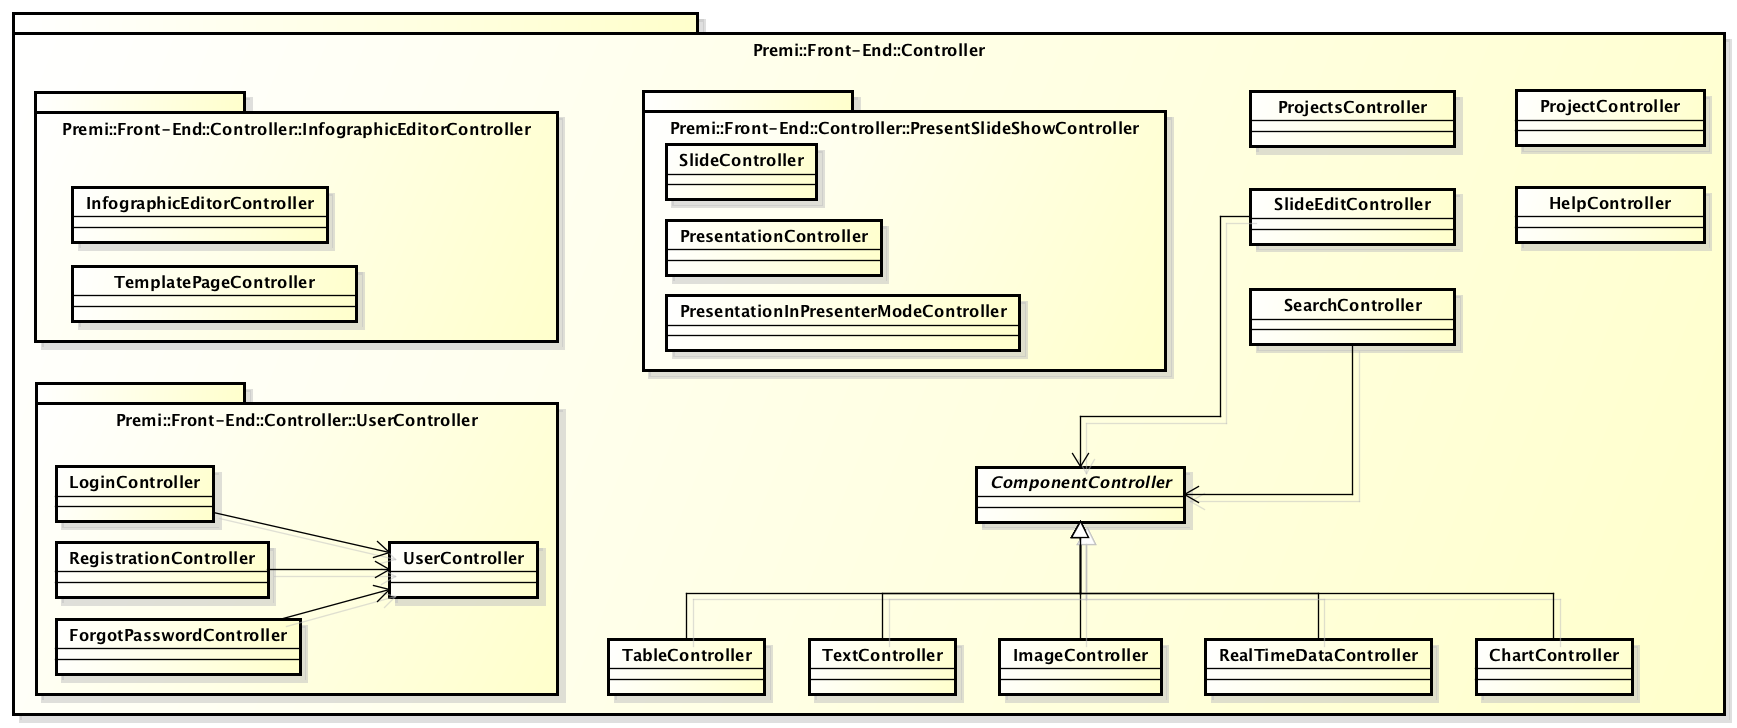
\includegraphics[width=1.0\linewidth]{img/front-end_controller}
	\caption[Premi::Front-End::Controllers]{Premi::Front-End::Controllers}
\end{figure}
\begin{itemize}
	\item \textbf{Descrizione}: Il package serve a far comunicare le view con il model in entrambe le direzioni ovvero rendere visibili gli aggiornamenti del model nella view e viceversa aggiornare il model con le informazioni provenienti dalla view.
	\item \textbf{Interazione con altri package}:
	\begin{itemize}
		\item Vi è un'interazione con il package Premi::Front-End::Views in quanto i controller sono utilizzati per iniziallizzare le view e per aggiornare il model del frontend con le modifiche avvenute in esse;
		\item Vi è un'interazione con il package Premi::Front-End::Model poiché in esso vengono depositati e prelevati i dati necessari alle view richieste;
		\item Vi è un'interazione con il package Premi::Front-End::Services responsabile del recupero e salvataggio delle informazioni e dell'invocazione di precise procedure dall'esterno mediante chiamate REST.
	\end{itemize}

\end{itemize}

\subsubsection*{Classi contenute}
\begin{itemize}

	\item Premi::Front-End::Controllers::ProjectsController:
	\begin{itemize}
		\item \textbf{Descrizione}: classe con lo scopo di fornire le operazioni necessarie alla visualizzazione e gestione dei progetti relativi ad un utente.
		\item \textbf{Relazioni con altre classi}:
		\begin{itemize}
			\item Premi::Front-End::Services::ProjectService.
		\end{itemize}
	\end{itemize}
	\item  Premi::Front-End::Controllers::ProjectController:
	\begin{itemize}
		\item \textbf{Descrizione}: classe con lo scopo di fornire le operazioni necessarie alla gestione di un progetto.
		\item \textbf{Relazioni con altre classi}:
		\begin{itemize}
			\item Premi::Front-End::Services::ProjectService.
		\end{itemize}
	\end{itemize}
	\item  Premi::Front-End::Controllers::SlideEditorController:
	\begin{itemize}
		\item \textbf{Descrizione}: classe di suporto all'editor di una presentazione fornendo le operazioni necessarie alla composizione e modifica di una slide. Essa permette di assemblare e modificare una \gls{slide} e i metodi che effettueranno le operazioni sui componenti.
		\item \textbf{Relazioni con altre classi}:
		\begin{itemize}
			\item Premi::Front-End::Controllers::ComponentController;
			\item Premi::Front-End::Services::SlideService.
		\end{itemize}
	\end{itemize}
	\item  Premi::Front-End::Controllers::PresentationEditorController:
	\begin{itemize}
		\item \textbf{Descrizione}: classe con lo scopo di fornire le operazioni necessarie alla gestione dell'editor di una presentazione. Essa permette di assemblare e modificare una \gls{slide} e i metodi che effettueranno le operazioni sui componenti.
		\item \textbf{Relazioni con altre classi}:
		\begin{itemize}
			\item Premi::Front-End::Controllers::SlideEditorController;
			\item Premi::Front-End::Services::PresentationService.
		\end{itemize}
	\end{itemize}
	\item  Premi::Front-End::Controllers::InfographicEditorController:
	\begin{itemize}
		\item \textbf{Descrizione}: classe con lo scopo di fornire le operazioni necessarie alla gestione dell'editor di una inforgrafica. Essa permette di assemblare e modificare una \gls{slide} e i metodi che effettueranno le operazioni sui componenti.
		\item \textbf{Relazioni con altre classi}:
		\begin{itemize}
			\item Premi::Front-End::Services::InfographicService.
		\end{itemize}
	\end{itemize}
	\item  Premi::Front-End::Controllers::ComponentController:
	\begin{itemize}
		\item \textbf{Descrizione}: classe con lo scopo di fornire le operazioni necessarie alla gestione di un componente di una \gls{slide}.
	\end{itemize}
	\item  Premi::Front-End::Controllers::PresentationController:
	\begin{itemize}
		\item \textbf{Descrizione}: classe con lo scopo di fornire le operazioni necessarie alla gestione della visualizzazione di una presentazione. Essa permette di assemblare e configurare una presentazione e di rendere disponibile la visualizzazione in modalità classica o presentatore.
		\item \textbf{Relazioni con altre classi}:
		\begin{itemize}
			\item Premi::Front-End::Services::PresentationService.
		\end{itemize}
	\end{itemize}
	\item  Premi::Front-End::Controllers::LoginController:
	\begin{itemize}
		\item \textbf{Descrizione}: classe con lo scopo di fornire le operazioni necessarie all'autenticazione nel sistema.
		\item \textbf{Relazioni con altre classi}:
		\begin{itemize}
			\item Premi::Front-End::Services::AuthenticationService.
		\end{itemize}
	\end{itemize}
	\item  Premi::Front-End::Controllers::SignUpController:
	\begin{itemize}
		\item \textbf{Descrizione}: classe con lo scopo di fornire le operazioni necessarie alla registrazione di un nuovo utente nel sistema.
		\item \textbf{Relazioni con altre classi}:
		\begin{itemize}
			\item Premi::Front-End::Services::AuthenticationService.
		\end{itemize}
	\end{itemize}
	\item  Premi::Front-End::Controllers::SearchController:
	\begin{itemize}
		\item \textbf{Descrizione}: classe con lo scopo di fornire le operazioni necessarie alla ricerca di progetti e presentazioni mediante il titolo oppure il nome.
		\begin{itemize}
			\item Premi::Front-End::Services::ProjectService.
		\end{itemize}
	\end{itemize}
	\item  Premi::Front-End::Controllers::HelpController:
	\begin{itemize}
		\item \textbf{Descrizione}: classe con lo scopo di fornire le operazioni necessarie alla gestione dell'aiuto agli utenti sottoforma di tour\footnote{Un tour è una esplorazione guidata delle funzionalità basilari del sistema al fine di permettere all'utente di familiarizzare velocemente con esso.} e suggerimenti.
	\end{itemize}
\end{itemize}
\newpage


		\subsection{Premi::Front-End::Views}
				\subsubsection*{Informazioni sul package}
		\begin{figure}[h]
			\centering
			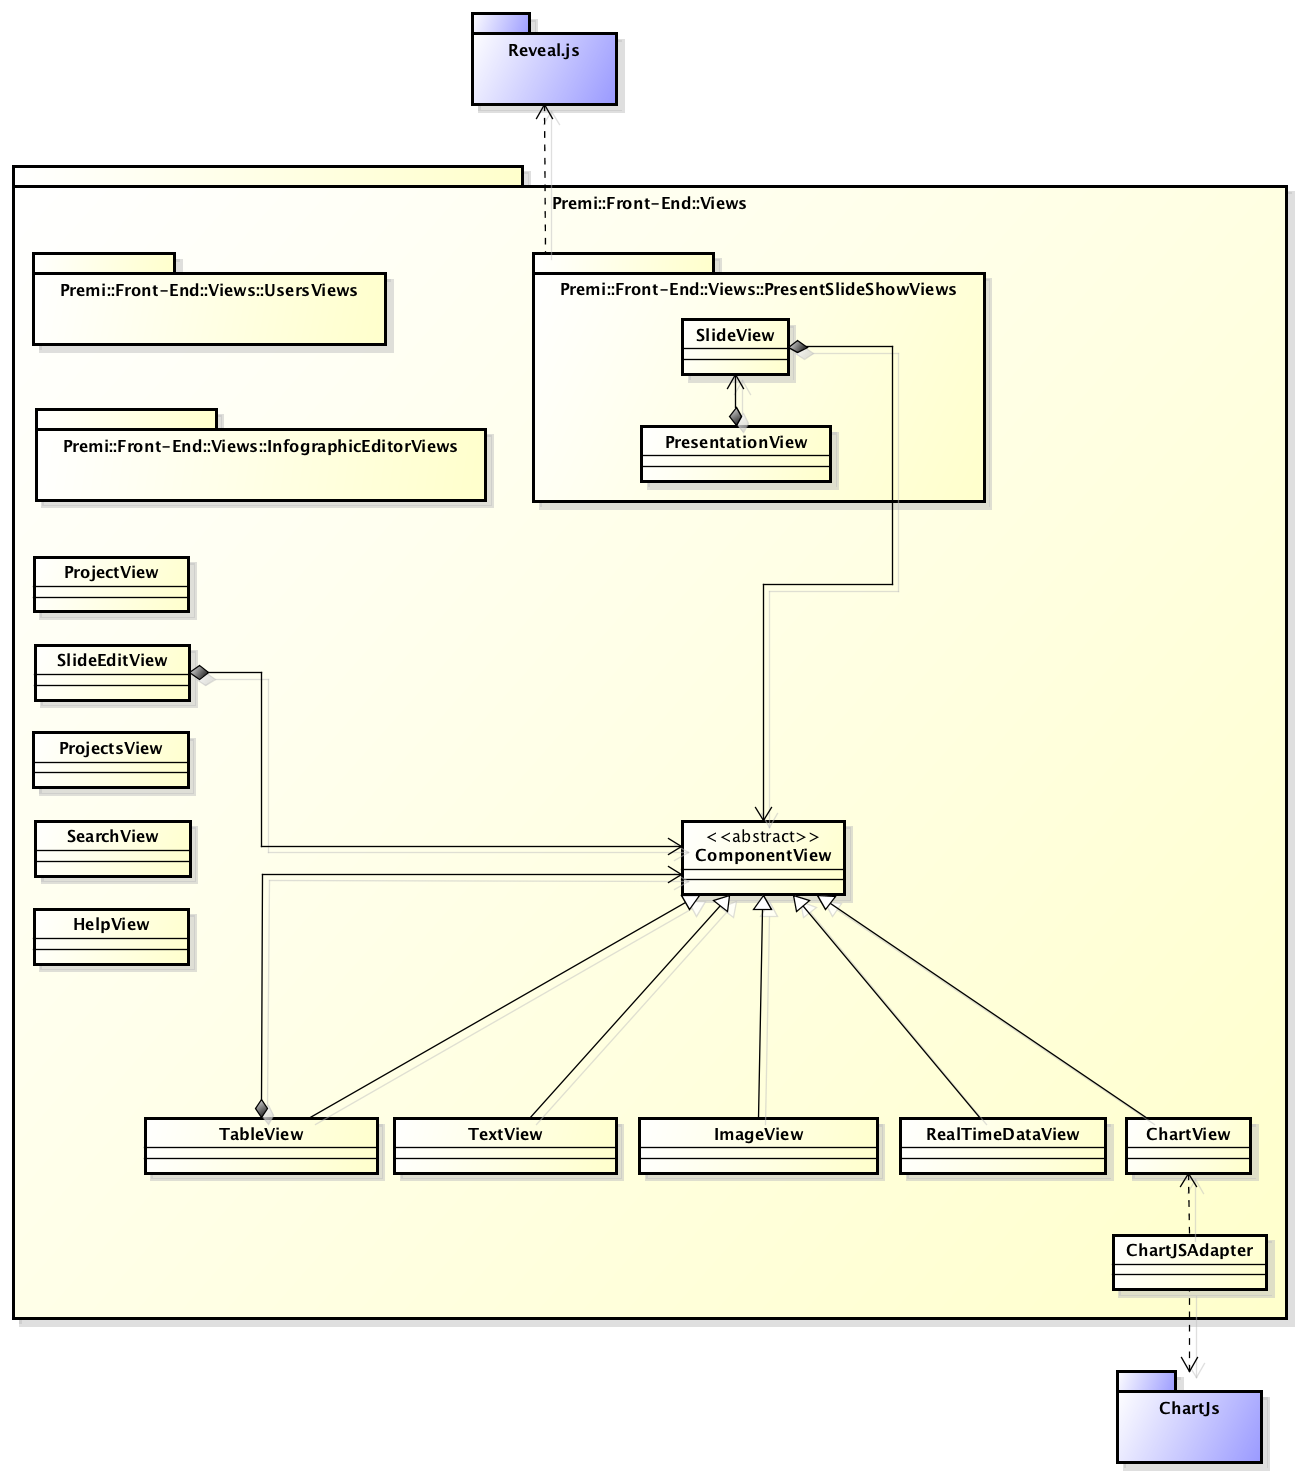
\includegraphics[width=0.7\linewidth]{img/front-end_views}
			\caption[Premi::Front-End::Views]{Premi::Front-End::Views}
		\end{figure}
		Il package contiene gli elementi per creare la parte grafica del \gls{front-end}, la visualizzazione delle pagine e dell'editor del progetto.

	\subsubsection*{Package contenuti:}

	\begin{itemize}
		\item Premi::Front-End::Views::UsersViews:
			\begin{itemize}
				\item \textbf{Descrizione}: classe per la gestione delle pagine riguardanti l'accesso al sito.
			\end{itemize}

		\item Premi::Front-End::Views::PresentSlideShowViews:
			\begin{itemize}
				\item \textbf{Descrizione}: classe per la gestione delle pagine per la visualizzazione della presentazione.
			\end{itemize}

		\item Premi::Front-End::Views::InfographicsEditorViews:
		\begin{itemize}
			\item \textbf{Descrizione}: classe per la gestione delle infografiche relative al progetto.
		\end{itemize}
	\end{itemize}

	\subsubsection*{Classi contenute:}
	\begin{itemize}

		\item Premi::Front-End::Views::UsersViews:
		\begin{itemize}
			\item \textbf{Descrizione}: classe per la gestione delle pagine riguardanti l'accesso al sito.
		\end{itemize}

		\item Premi::Front-End::Views::ProjectView:
		\begin{itemize}
			\item \textbf{Descrizione}: classe per la gestione della pagina del progetto attualmente aperto dall'utente.
		\end{itemize}

		\item Premi::Front-End::Views::SlideEditView:
		\begin{itemize}
			\item \textbf{Descrizione}: classe per la gestione della pagina dell'editor di una \gls{slide};
			\item \textbf{Relazioni con altre classi}:
			\begin{itemize}
				\item Premi::Front-End::Views::ComponentView.
			\end{itemize}
		\end{itemize}

		\item Premi::Front-End::Views::ProjectsView:
		\begin{itemize}
			\item \textbf{Descrizione}: classe per la gestione della pagina contenente i progetti creati da un utente.
		\end{itemize}

		\item Premi::Front-End::Views::SearchView:
		\begin{itemize}
			\item \textbf{Descrizione}: classe per la gestione della pagina per la ricerca di un progetto e la visualizzazione dei risultati.
		\end{itemize}

		\item Premi::Front-End::Views::HelpView:
		\begin{itemize}
			\item \textbf{Descrizione}: classe per la gestione della pagina della guida dell'applicazione.
		\end{itemize}

		\item Premi::Front-End::Views::ComponentView:
		\begin{itemize}
			\item \textbf{Descrizione}: classe base per la gestione grafica degli elementi che è possibile includere in una \gls{slide}.
		\end{itemize}

		\item Premi::Front-End::Views::TableView:
		\begin{itemize}
			\item \textbf{Descrizione}: classe per la gestione grafica dell'elemento tabella che è possibile includere in una \gls{slide}. Può essere composta da altri elementi della classe *::ComponentView;
			\item \textbf{Relazioni con altre classi}:
			\begin{itemize}
				\item Premi::Front-End::Views::ComponentView.
			\end{itemize}
		\end{itemize}


		\item Premi::Front-End::Views::TextView:
		\begin{itemize}
			\item \textbf{Descrizione}: classe per la gestione grafica dell'elemento casella di testo che è possibile includere in una \gls{slide};
			\item \textbf{Relazioni con altre classi}:
			\begin{itemize}
				\item Premi::Front-End::Views::ComponentView.
			\end{itemize}
		\end{itemize}

		\item Premi::Front-End::Views::ImageView:
		\begin{itemize}
			\item \textbf{Descrizione}: classe per la gestione grafica dell'elemento immagine che è possibile includere in una \gls{slide};
			\item \textbf{Relazioni con altre classi}:
			\begin{itemize}
				\item Premi::Front-End::Views::ComponentView.
			\end{itemize}
		\end{itemize}

		\item Premi::Front-End::Views::RealTimeDataView:
		\begin{itemize}
			\item \textbf{Descrizione}: classe per la gestione grafica dell'elemento di dati real-time che è possibile includere in una \gls{slide};
			\item \textbf{Relazioni con altre classi}:
			\begin{itemize}
				\item Premi::Front-End::Views::ComponentView.
			\end{itemize}
		\end{itemize}

		\item Premi::Front-End::Views::ChartView:
		\begin{itemize}
			\item \textbf{Descrizione}: classe per la gestione grafica dell'elemento grafico che è possibile includere in una \gls{slide};
			\item \textbf{Relazioni con altre classi}:
			\begin{itemize}
				\item Premi::Front-End::Views::ComponentView;
				\item Premi::Front-End::Views::ChartJsAdapter;
			\end{itemize}
		\end{itemize}

		\item Premi::Front-End::Views::ChartJsAdapter:
		\begin{itemize}
			\item \textbf{Descrizione}: classe per interfacciare l'utilizzo della classe Chart.Js con la classe ChartView;
			\item \textbf{Relazioni con altre classi}:
			\begin{itemize}
				\item Premi::Front-End::Views::ChartView;
			\end{itemize}
			\item \textbf{Relazioni con altri package}:
			\begin{itemize}
				\item Chart.Js
			\end{itemize}
		\end{itemize}
	\end{itemize}


\subsection{Premi::Front-End::Views::UsersViews}
	\subsubsection*{Informazioni sul package}
	\begin{figure}[h]
		\centering
		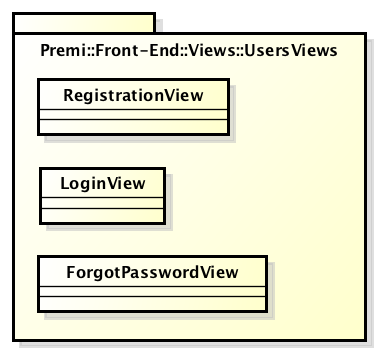
\includegraphics[width=0.7\linewidth]{img/front-end_views_usersviews}
		\caption[Premi::Front-End::Views::UsersViews]{Premi::Front-End::Views::UsersViews}
	\end{figure}
	Il package contiene le classi per creare la parte grafica dell'accesso di un utente all'applicazione.

	\subsubsection*{Classi contenute:}
	\begin{itemize}

		\item Premi::Front-End::Views::UsersViews::RegistrationView:
		\begin{itemize}
			\item \textbf{Descrizione}: classe per creare la sezione relativa alla registrazione di un nuovo utente.
		\end{itemize}

		\item Premi::Front-End::Views::UsersViews::LoginView:
		\begin{itemize}
			\item \textbf{Descrizione}: classe per creare la sezione relativa al login di utente già registrato.
		\end{itemize}

		\item Premi::Front-End::Views::UsersViews::ForgotPasswordView:
		\begin{itemize}
			\item \textbf{Descrizione}: classe per creare la sezione relativa al recupero della password per l'utente registrato.
		\end{itemize}
	\end{itemize}


\subsection{Premi::Front-End::Views::PresentSlideShowViews}
	\subsubsection*{Informazioni sul package}
	\begin{figure}[h]
		\centering
		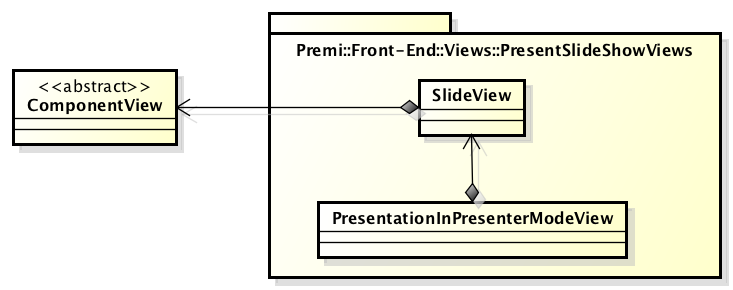
\includegraphics[width=0.7\linewidth]{img/front-end_views_presentslideshowviews}
		\caption[Premi::Front-End::Views::PresentSlideShowViews]{Premi::Front-End::Views::PresentSlideShowViews}
	\end{figure}
	Il package contiene le classi per la parte grafica relativa alla visualizzazione della presentazione da parte dell'utente.

	\subsubsection*{Classi contenute:}
		\begin{itemize}
			\item Premi::Front-End::Views::PresentSlideShowViews::SlideView:
			\begin{itemize}
				\item \textbf{Descrizione}: classe per creare la parte grafica di una \gls{slide} nella visualizzazione di una presentazione. È composta da oggetti della classe ComponentView,o sue derivate;
				\item \textbf{Relazioni con altre classi}:
				\begin{itemize}
					\item Premi::Front-End::Views::ComponentView.
				\end{itemize}
			\end{itemize}

			\item Premi::Front-End::Views::PresentSlideShowViews::PresentationInPresenterModeView:
			\begin{itemize}
				\item \textbf{Descrizione}: classe per creare la parte grafica di una \gls{slide} nella visualizzazione di una presentazione nella modalità presentatore. È composta da oggetti della classe SlideView in quanto la contiene implementandola;
				\item \textbf{Relazioni con altre classi}:
				\begin{itemize}
					\item Premi::Front-End::Views::PresentSlideShowViews::SlideView.
				\end{itemize}
			\end{itemize}
		\end{itemize}

\newpage
\subsection{Premi::Front-End::Views::InfographicEditorViews}
	\subsubsection*{Informazioni sul package}
	\begin{figure}[h]
		\centering
		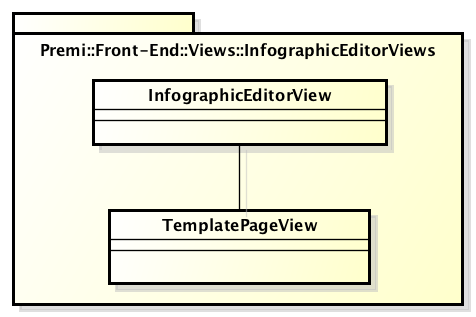
\includegraphics[width=0.7\linewidth]{img/front-end_views_infographiceditorviews}
		\caption[Premi::Front-End::Views::InfographicEditorViews]{Premi::Front-End::Views::InfographicEditorViews}
	\end{figure}
	Il package contiene le classi per la parte grafica relativa alle infografiche e alla loro creazione.

	\subsubsection*{Classi contenute:}
	\begin{itemize}

		\item Premi::Front-End::Views::InfographicEditorViews::InfographicEditorView:
		\begin{itemize}
			\item \textbf{Descrizione}: classe per creare un'\gls{infografica}. Permette la personalizzazione di essa attraverso la selezione delle \gls{slide} da usare.
		\end{itemize}

		\item Premi::Front-End::Views::InfographicEditorViews::TemplatePageView:
		\begin{itemize}
			\item \textbf{Descrizione}: classe che permette di creare la sezione per selezionare il \gls{template} da utilizzare nell'\gls{infografica};
			\item \textbf{Relazioni con altre classi}:
			\begin{itemize}
				\item Premi::Front-End::Views::InfographicEditorViews::InfographicEditorView.
			\end{itemize}
		\end{itemize}
	\end{itemize}

